\documentclass[template.tex]{subfiles}

\usepackage{comment} 

\begin{document}

\begin{comment}
Andrew's comments: (THIS IS METHODS)
- describe modelling framework and details how you built everything
- now explain in detail what the package is \& can do, what the structure is like
- clarify that it is situated in complexity between custom scripts and modelling tools with graphical interfaces. It would be possible to design a graphical interface for this later on, but that is not the target audience.


"Python is a high-level programming language well suited to rapid development and prototyping, as well as being more accessible to domain scientists than low-level languages such as FORTRAN or C++." - Mobius GMD paper
- This is also due to the dynamic interpretation of python, which makes python slower, but python is rapidly developing and leveraging other lower level language for speed. Also has high functionality for parallelisation of code execution which is very relevant to complex marine ecosystem models. 

- clearly state limitations (scope) of phydra 
- mention that xarray-simlab is general enough to support IBMs! But not developed here.
\end{comment}



 %% \ SECTION 2
\section{The Phydra package: structure \& features} \label{Section:phydrapackage}
% 2nd Section:
% Background, theoretical framework. Specifics here!


Phydra is an open-source object-oriented Python package for modeling marine ecosystems.



The goal of this project is to support efficient, open and easily reproducible model development. 

\subsection{Python backend: xarray-simlab and GEKKO}

The Phydra package is built using the wealth of functionality provided by the open-source scientific Python community. Two packages in particular form the basis of Phydra: Xarray-simlab as a flexible framework and GEKKO as an efficient solver.

GEKKO as a computational backend.

The library of modular processes and the user interface are built from the xarray-simlab package \citep{Bovy2018Xarray-simlab:Interactively}. 
Xarray-simlab provides a generic framework for building computational models in a modular fashion and an extension for model setup, running simulations and storing output using the xarray.Dataset structure.

Xarray provides an efficient and labelled multi-dimensional storage format, that is integrated with functionality for easy plotting and post-processing and storing of model output. Xarray.Datasets are easily converted to Netcdf files, the commonly used file format for biogeochemical data. 

In addition to a native storage format, xarray-simlab provides the object-oriented framework for model building blocks, as well as the model setup and runtime user interface in Phydra. A process that is part of the model is 

Xarray-simlab currently only provides step-wise calculation of Python functions acting on defined variables and is not optimised for solving systems of differential equations. Instead we use the Python GEKKO Optimisation suite to provide a more robust back end to solving models built in Phydra. GEKKO is an open-source, object-oriented library of model construction, analysis and optimisation tools built on a core algebraic modelling language \citep{Beal2018GEKKOSuite}. Models can be constructed based on a common syntax and are compiled to efficient FORTRAN code before solving.
Utilizing GEKKO as a backend solver within the xarray-simlab framework, we can combine the usability of a high-level language like Python with the efficient computation of lower-level languages.

Both of these Python packages are relatively young and actively being developed, which provides some challenges but also allows for constant improvements to the functionality that Phydra provides.
Below we will describe how Phydra leverages these open-source projects to provide a tool-set to construct, modify, solve, analyse and share marine ecosystem models. The basic modular components of Phydra are discussed and a general model development workflow is presented.


\subsection{Phydra building-blocks}

Phydra leverages the objects and syntax provided by the xarray-simlab and GEKKO packages, to create a set of building-blocks for ecosystem models that can be combined flexibly. 

Phydra provides a library of modular model building-blocks that can be used to assemble complex marine ecosystem models. These building-blocks are contained in xarray-simlab processes, which are specially decorated Python classes.

When assembling a model, there are certain basic processes that have to be included in order to allow the GEKKO solver to assemble the full model. These base processes are included with every call to create a Phydra model using \texttt{phydra.Model()}. Additional processes to add to the model can be drawn from the Phydra library. 
The library is ordered into different logical components in a marine ecosystem, describing their function either as an environment, component, flux or forcing. 

The logic behind this order is that an ecosystem model would need at least one of each of these processes added in order to run. Phydra currently only supports running a single environment in a 0-dimensional setting with a flexible number of components and fluxes. In future versions the framework can potentially support multiple environments and dimensions.

The open-source code structure allows users to easy develop or modify processes to describe a specific ecosystem. The ordering of the building-blocks is not an implicit order, self-written building blocks can blur the boundaries and combine different functions.

The first version of the library will contain all processes needed to create the three model use cases presented in Section \ref{Section:UseCases}. Users of Phydra could provide their own use cases to the standard library in a collaborative effort to support efficient, open and easily reproducible marine ecosystem model development.

As a collaborative process, the library can grow to incorporate a much wider range of use cases.

These processes are classes that are provided with Phydra. We separate the processes into multiple logical categories that represent structures in a marine ecosystem model: Environments, Forcings, Components and Fluxes.

\subsubsection{Environments} \label{Section:PhysicalEnvironment}

A Phydra Environment defines the structure of the ecosystem and provides external inputs (i.e. forcings) that can be accessed by all processes linked to this environment. As a simple example we could take a chemostat model. The flow-through culture system is defined by a solution of nutrients that flows into a tank of fixed volume. Organisms within the tank grow, consume nutrients and are also flushed out of the system with the outflow of the medium. The Environment process in Phydra describing a chemostat would have the nutrient concentration in the medium, as well as the flow-rate of the system as required external forcing processes. The forcing input can be supplied from different Forcing processes, for example with a time-varying flow rate. Components, which define the state variables in our model, are grouped within our chemostat Environment and the Fluxes (e.g. nutrient uptake or mortality) affect Components within this Environment. We can add any number of Components from the Phydra library into our Environment and between the Components we could add any number of interactions.

Phydra as of now provides an easily modifiable base Environment and implementations of a chemostat Environment, as well as a slab-ocean Environment. The first release of Phydra supports only single zero-dimensional implementations of these basic ecosystem models, but the development of multi-dimensional Environments is a high priority for further development.

\subsubsection{Forcings} \label{Section:ForcingSection}

Model forcings and data used in model optimisation are represented by GEKKO parameters that are supplied to the model discretised at the same time-step that the model is solved.

Included with this version of Phydra we have the necessary forcing types that have to be supplied to the provided Environments. For a chemostat model, this is a source concentration of a component in the medium, as well as a flow rate of the system. The slab-ocean Environment interfaces with forcings describing the concentration of a component below the mixed layer, movement of the mixed layer depth (MLD), irradiance at surface and temperature within the mixed layer. There are basic methods supplied to create either constant forcing or values over time based on mathematical functions. Additionally a base Forcing process can be modified by a user to provide any external data, which can then be used by other processes in the library. The flexible class-based structure allows a process class inheriting from the base MLD forcing process to be recognised as an MLD forcing in the Fluxes and processes of our model.

\subsubsection{Components}

An ecosystem model tracks chemical compounds as well as organisms via state variables. These state variables can define completely different components of a model, or represent a functional group. Components within Phydra are defined at this higher level and can contain a single state variable or an array of state variables that share common fluxes with differing parameterisation. Each component is added to the model with a specific label that is used to reference this component in all processes affecting or dependent on it. 

The actual dimensions of a model component are initialized after passing a parameter at model setup. 

This has been designed for easily testing different levels of ecosystem complexity. As shown in the second use case, where this is useful is in setting up phytoplankton size classes in trait-based models. All phytoplankton state variables grow on a common nutrient, but uptake parameters are related to allometries of cell size. A phytoplankton component could be initialized, with a certain size range and number of state variables. Within the allometric growth process parameters are dynamically initialized based on the size provided by the component. 

Phydra thus simplifies model setup for these types of models considerably. 

In addition to size, the component could be modified to include information on units or other specific parameters relevant to the model. The added flexible dimensionality of components was designed with the current issues in marine ecosystem model in mind. The effects of different levels of complexity, in the number and definition of phytoplankton functional types (PFT) for example, is not routinely tested in marine ecosystem models. Phydra provides a framework that allows for easy testing through flexible modification of such model complexity at model setup.

Components in Phydra currently only supports 1-dimensional functional groups, but extending this to 2- and 3-dimensional flexibility is a high development priority. 


\subsubsection{Fluxes}
The previous building blocks of an environment, components and forcing create the structure of the model, but when solved at this stage there would be no meaningful simulation. In order to define exchanges of matter between components flux processes are added to our model instance, defining the affected components via labels at model setup.
There are multiple types of fluxes provided as base classes in the library. These base classes are defined by the type of interaction between components. Single fluxes provide loss or gain processes to a single variable, such as sinking or influx from outside the ecosystem. In order to simplify creating common forcing fluxes, a single flux process can a list of affected components as input at model setup. An example for more complex forcing type are exchange fluxes, where a flux affects one component as a source and another as a sink. These can be set up with flexible dimensionality of components. Grazing fluxes are a slightly more complicated subclass of a grid-wise flux, as ingestion is usually normalized by total prey availability, so all forcing interactions need to be calculated in a dynamically generated matrix of all prey items consumed by a component.

Will be able to develop much further, extending flux base classes or adding new ones.


- Flows are parts of differential equations, that affect one or more components, and can be influenced by forcing and the physical environment


\subsubsection{Installing and running Phydra}
The Phydra package is available via the Python pip package manager, but we encourage using Conda as a package manager that is provided with the scientific Anaconda Python distribution.
Please follow the up-to-date instructions on the Github repository for installation of Phydra and its dependencies.
% CONDA NAME DROP
Since python is a fast developing language, we will provide instructions to install a fully compatible virtual environment with the Conda package manager separate from a users normal python environment. For interactive coding and rapid prototyping we recommend using the Jupyter environment that is available via Conda. For more complex and larger model runs on servers or clusters python scripts are preferable.

\subsection{Model development workflow}

The model construction process has two definitive stages, 
 
 \texttt{phydra.Model()}
 
 \texttt{phydra.create_setup()}

Constructing marine ecosystem models in Phydra is by nature flexible, but the user can follow a general workflow of assembling models from the library of processes. This wokflow is visualized in \ref{Figure:phydraschematics} and will be further explained below.

\subsubsection{Model construction}
Here 
- Dimensionality is a very important fact of building models, and xarray-simlab provides a simple, but sometimes tricky interface for managing dimensionality, so make sure to explain it relatively well here, as well as the implementations.
- I can cite https://www.biogeosciences.net/17/609/2020/ to explain why dimensionality is an important consideration in phytoplankton models.

\subsubsection{Runtime}
- explain what the options are to run the model, depends on if a time implicit method will be added to solve, or if it will just remain with the time explicit steps of xarray-simlab

\subsubsection{Model Diagnostics}
- this is a relevant section, *if* Benoît can help me with creating the ODE visualisation & model diagnostics.

\subsubsection{Parameter fitting}
- this is a relevant section, if i manage to get some decent parameter fitting results for the example 1 and 3.. either only 3 or both, is my feeling. 


\subsubsection{Modification and further development}

- Similar to how a forcing process can easily be subclassed to supply a different forcing, other processes in xsimlab can be easily subclassed and modified to have a different function, as long as the interaction between state variables matches
- Explain interface to process subclasses, and how it is relatively easy to set up xsimlab processes with slightly different  formulations, but the same basic interaction

% OPEN SOURCE CONTRIBUTION 
Phydra (like Xarray-simlab and GEKKO) is an open-source project. Contributions are welcome and in fact greatly appreciated. You can contribute in many ways by reporting bugs, submitting feedback, contributing to the development of the code or the documentation for example. Please read the contributing guidelines on the Github repository for further details.





%%% TWO-COLUMN FIGURES
%
%%f
\begin{figure*}[t]
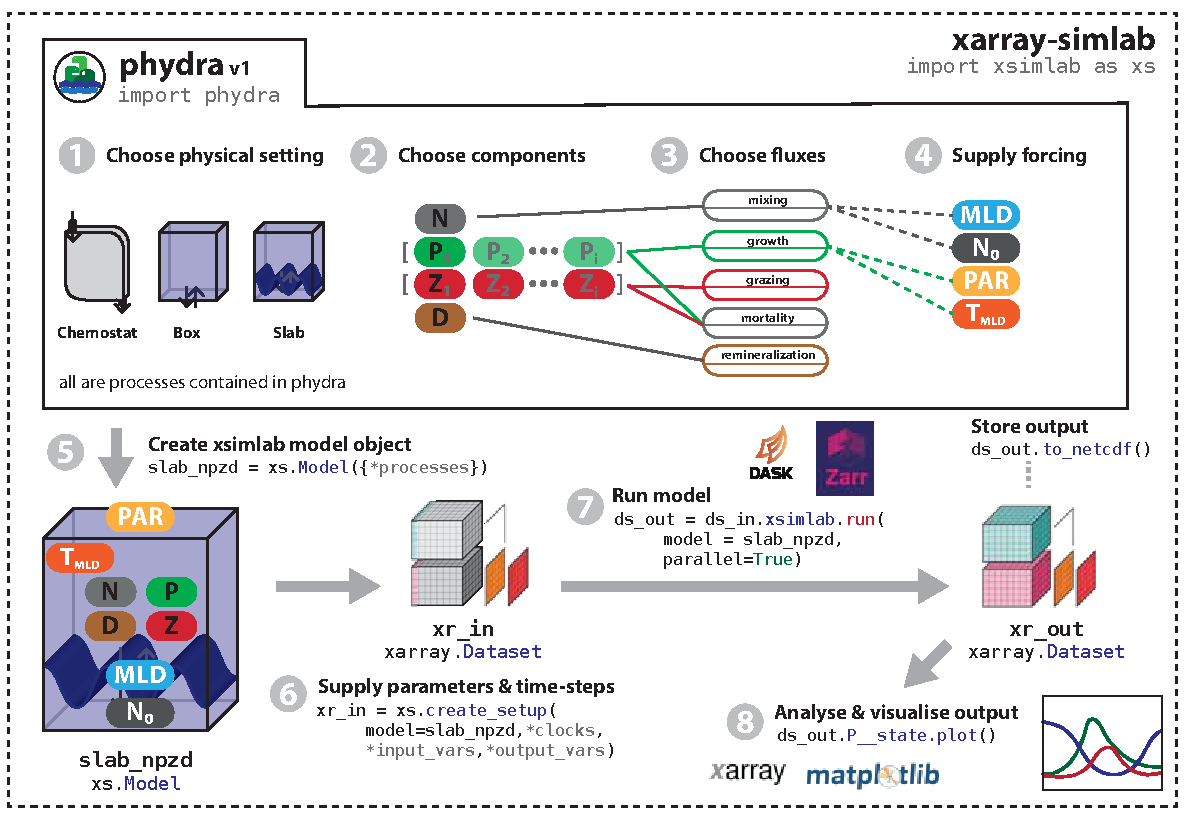
\includegraphics[width=12cm]{Figures/firstdraft_schematics/01__schematics_phydra_1.pdf}
\caption{The phydra package is embedded within the xarray-simlab framework. phydra contains a library of physical settings (1), components (i.e. state variables) (2), fluxes (3) and forcing variables (4), that can be combined and reused to create an xarray-simlab model instance. Xarray-simlab provides the functionality to define the model (5) from processes in the phydra library, supply parameters and create an xarray input (6), then run the model (7) and the resulting output is dynamically stored in another xarray, with fully labelled dimensions and containing all parameters.}
\label{Figure:phydraschematics}
\end{figure*}

general explanation, and then go into detail below (see Figure \ref{Figure:phydraschematics})





% Everything below here is optional, it depends on what I can actually do in the package
% this is a custom function to be able to see references when rendering subfiles:
\biblio

\end{document}